\documentclass[a4paper,10pt]{article}
\usepackage[brazil]{babel}
\usepackage[utf8]{inputenc}
\usepackage[T1]{fontenc}
\usepackage{amsmath}
\usepackage{hyperref}
\usepackage{url}
\usepackage{graphicx}
\usepackage{subfigure}

    \usepackage{xcolor,listings}
    \usepackage{textcomp}
    \usepackage{color}

    \definecolor{codegreen}{rgb}{0,0.6,0}
    \definecolor{codegray}{rgb}{0.5,0.5,0.5}
    \definecolor{codepurple}{HTML}{C42043}
    \definecolor{backcolour}{HTML}{F2F2F2}
    \definecolor{bookColor}{cmyk}{0,0,0,0.90}  
    \color{bookColor}

    \lstset{upquote=true}

    \lstdefinestyle{mystyle}{
				language=SQL,
				deletekeywords={IDENTITY},
				deletekeywords={[2]INT},
				morekeywords={clustered},
				framesep=8pt,
				%xleftmargin=40pt,
				%framexleftmargin=40pt,
				frame=tb,
				framerule=0pt,
        backgroundcolor=\color{backcolour},   
        commentstyle=\color{codegreen},
        keywordstyle=\color{codepurple},
        numberstyle=\footnotesize\color{codegray},
        stringstyle=\color{codepurple},
        basicstyle=\footnotesize,
        breakatwhitespace=false,         
        breaklines=true,                 
        captionpos=b,                    
        keepspaces=true,                 
        numbers=left,                    
        numbersep=-10pt,                  
        showspaces=false,                
        showstringspaces=false,
        showtabs=false,      
    }
    \lstset{style=mystyle} 

\title{Sistema de Cinema}
\author{
Felipe Luís Pinheiro - 18/0052667 \and 
João Pedro C.N. Mota - 17/0106144 \and 
Pedro Catelli - 17/0112624 \and
Pedro Oliveira - 17/0163768}

\begin{document}

\maketitle
%\makeindex

\begin{abstract}
Neste relatório desenvolvemos os requisitos básicos de um sistema de banco de dados para um modelo de vendas de ingresso de um cinema. 

Link para o repositório: \url{https://github.com/flpinheiro/banco_de_dados}. 
\end{abstract}

\section{Introdução}

Requisitos gerais:

\begin{itemize}
	\item Um cinema pode ter muitas salas, sendo necessário, por tanto, registrar informações a respeito de cada uma, como sua capacidade, ou seja, o numero de assentos disponíveis.
	\item O cinema apresenta muitos filmes. Um filme tem informações, titulo e duração. Assim, sempre que um filme for ser apresentado, deve-se registrá-lo também.
	\item Um mesmo filme pode ser apresentado em diferentes salas e em horários diferentes. Cada apresentação em uma determinada sala e horário é chamada sessão. Um filme sendo apresentado em uma sessão tem um conjunto máximo de ingressos, determinado pela capacidade da sala.
	\item Os clientes do cinema podem comprar ou não ingressos para assistir a uma sessão. O
funcionário deve intermediar a compra do ingresso. Um ingresso deve conter informação
como o tipo de ingresso (Meio ingresso ou ingresso inteiro). Além disso, um cliente só pode
comprar ingressos para sessões ainda não encerradas.
\end{itemize}

\section{Diagrama de Entidade Relacionamento}

Na figura \ref{fig:mer} mostramos a primeira versão conceitual do sistema do

\begin{figure}[h]
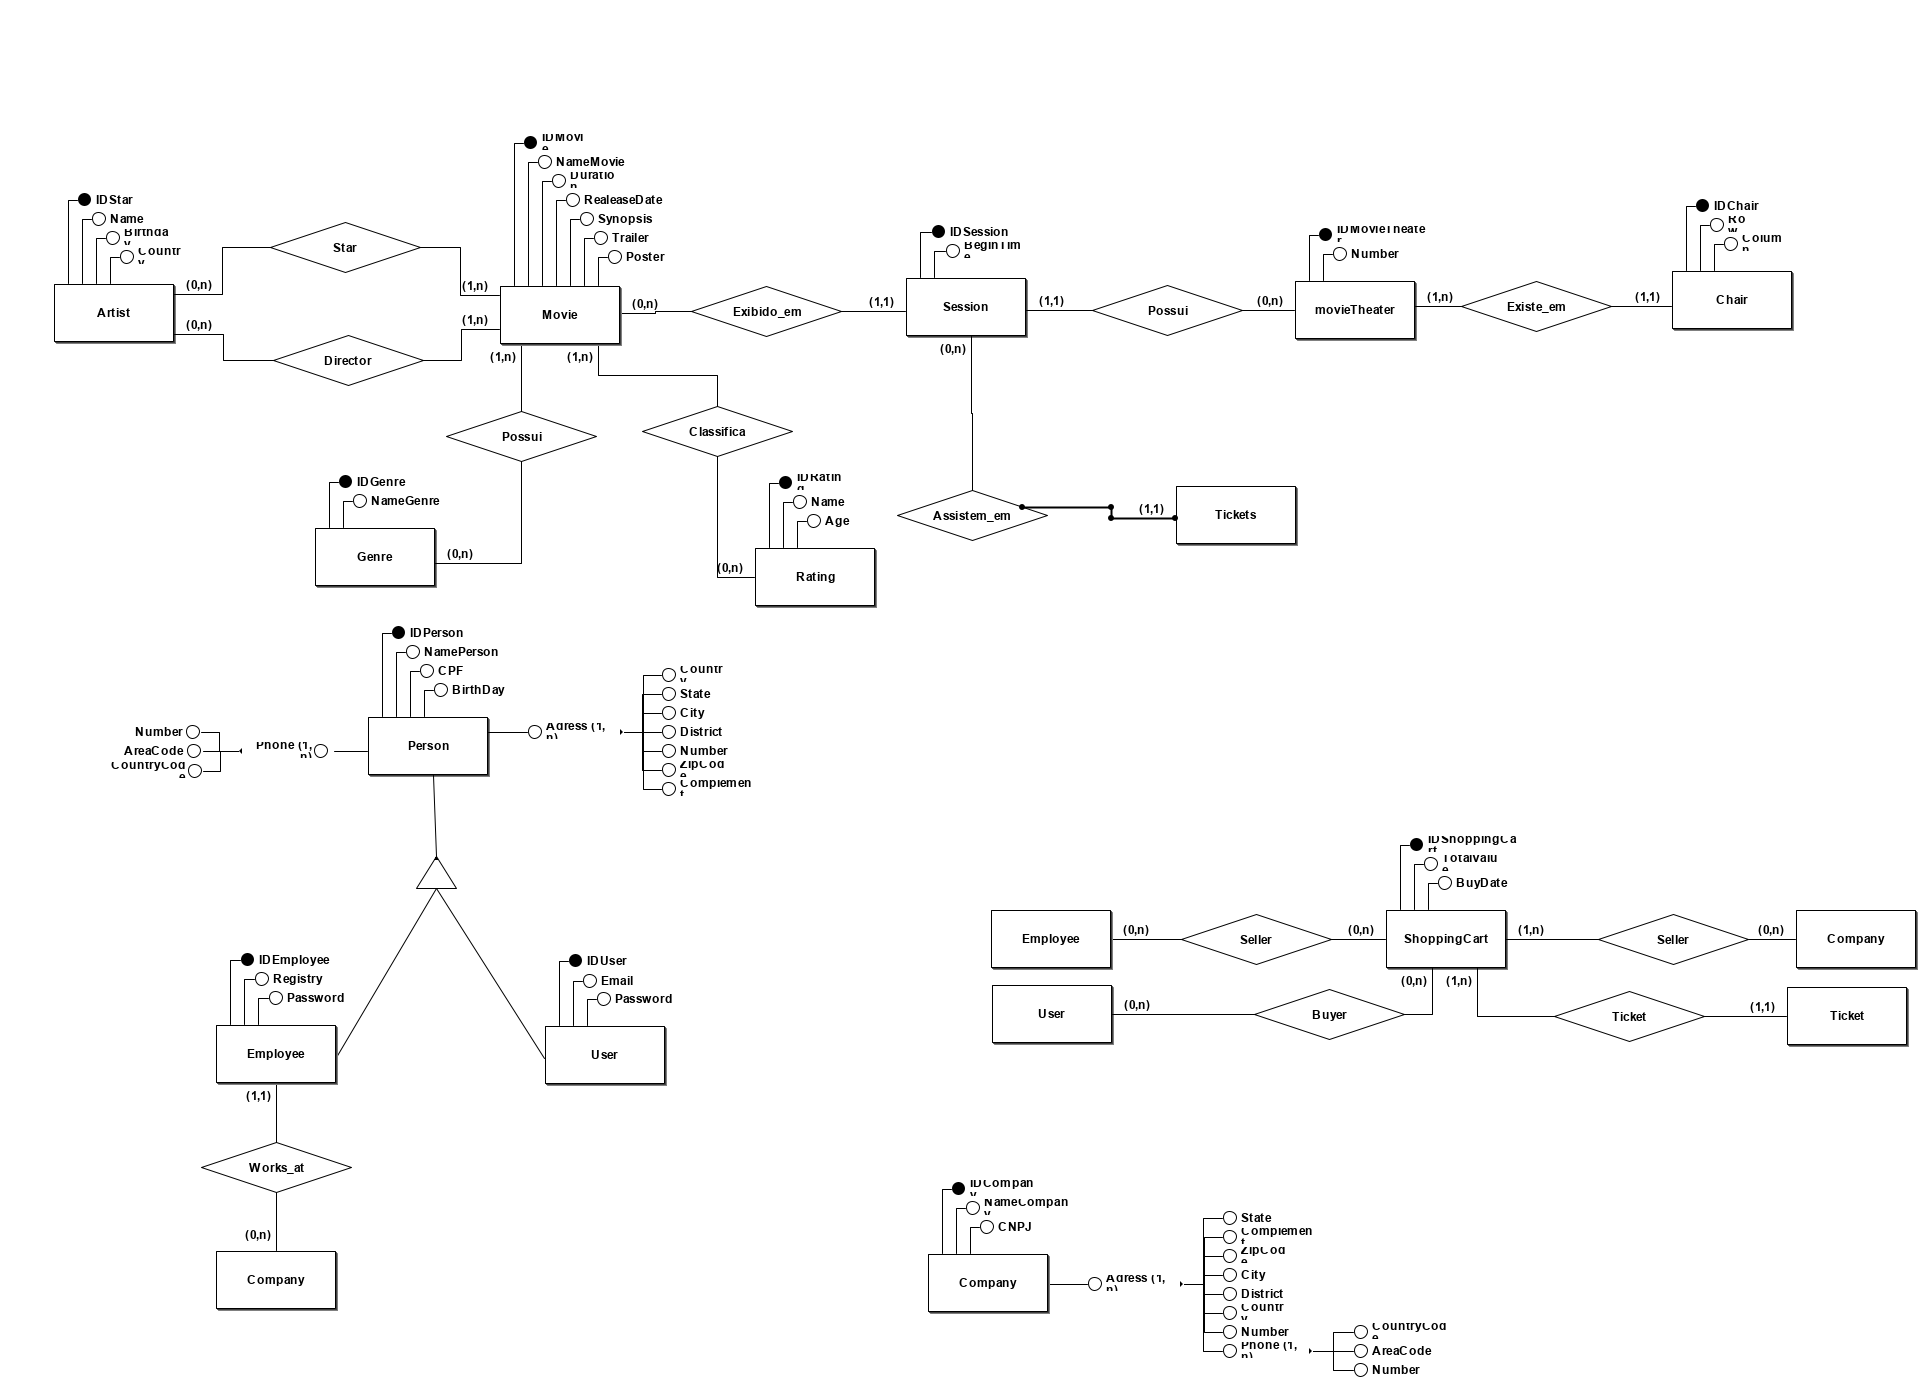
\includegraphics[width=\columnwidth]{UnBCineFlix_MER}%
\caption{Modelo Entidade Relacionamento}%
\label{fig:mer}%
\end{figure}

\section{Modelo Relacional}

Na figura \ref{fig:mr} mostramos o modelo relacional utilizado para implementação  do programa

\begin{figure}[h]
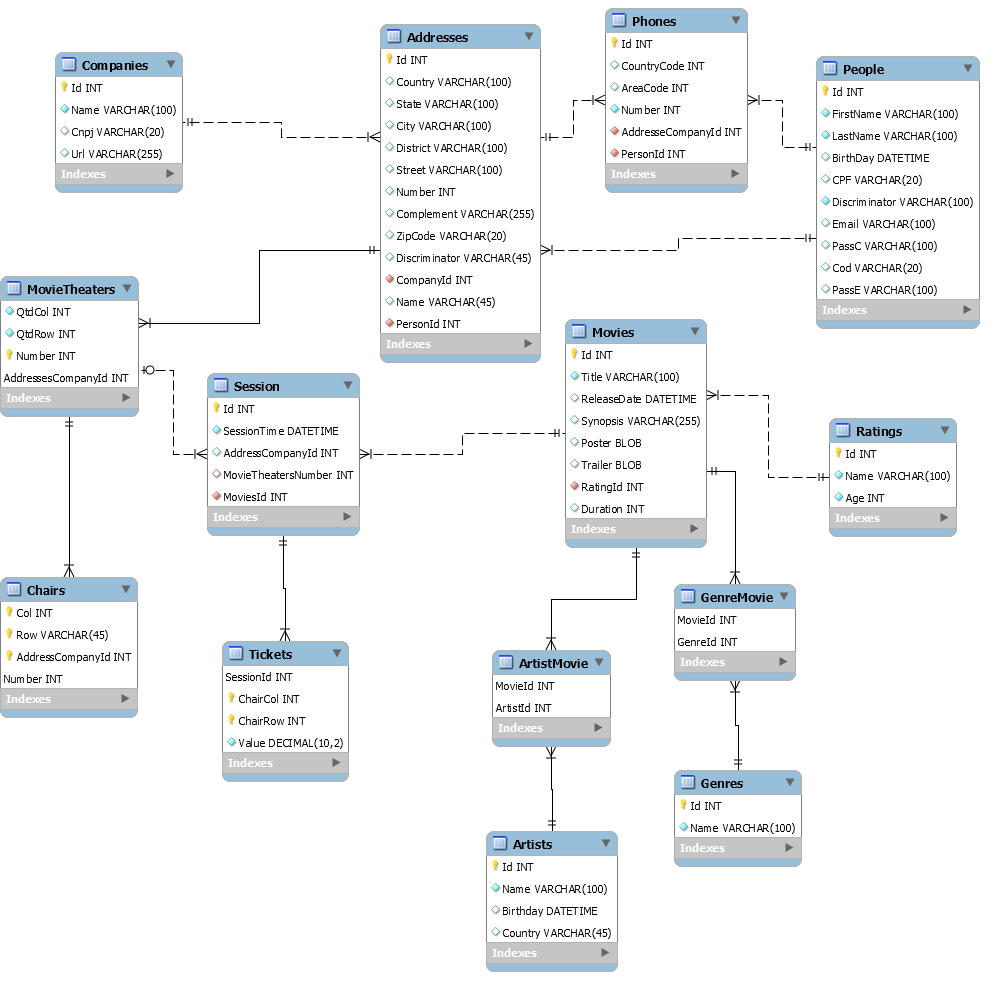
\includegraphics[width=\columnwidth]{UnBCineFlix_MR}%
\caption{Modelo Relacional}%
\label{fig:mr}%
\end{figure}

\section{Consultas}

Nesta seção mostramos exemplo de consultas que podem ser realizadas nesse modelo relacional de banco de dados.

\begin{lstlisting}
		use unbcineflix;
		
		select * FROM movies, ratings, genremovies, genres where ratingid = ratings.id and movies.id = genremovies.movieid and genremovies.genreid = genres.id;
		
		select * from movies, artistmovies, artists where Movies.id = artistmovies.MovieId and artistmovies.ArtistId = artists.Id;
		
		select * from movietheaters, addresses,companies where addresses.Id = movietheaters.AddressCompanyId and addresses.CompanyId = companies.Id and addresses.Discriminator = 'AddressCompany';
		
		select * from session, movietheaters, tickets where session.Id = tickets.SessionId and session.AddressCompanyId = movietheaters.AddressCompanyId and movietheaters.MovieTheaterNumber = session.MovieTheaterNumber;
		
		select * from people, addresses,phones where people.id = addresses.PersonId and people.id = phones.PersonId and addresses.Discriminator = 'AddressPerson';
\end{lstlisting}

\section{Script Sql}

Nesta seção mostramos o script sql para geração do banco de dados, que foi gerado utilizando o modelo acima e foi gerado automaticamente pelo MySQL.

\begin{lstlisting}
		-- MySQL Script generated by MySQL Workbench
		-- Thu Jun 27 18:36:45 2019
		-- Model: New Model    Version: 2.0
		-- MySQL Workbench Forward Engineering

		SET @OLD_UNIQUE_CHECKS=@@UNIQUE_CHECKS, UNIQUE_CHECKS=0;
		SET @OLD_FOREIGN_KEY_CHECKS=@@FOREIGN_KEY_CHECKS, FOREIGN_KEY_CHECKS=0;
		SET @OLD_SQL_MODE=@@SQL_MODE, SQL_MODE='ONLY_FULL_GROUP_BY,STRICT_TRANS_TABLES,NO_ZERO_IN_DATE,NO_ZERO_DATE,ERROR_FOR_DIVISION_BY_ZERO,NO_ENGINE_SUBSTITUTION';

		-- -----------------------------------------------------
		-- Schema UnBCineFlix
		-- -----------------------------------------------------
		DROP SCHEMA IF EXISTS `UnBCineFlix` ;

		-- -----------------------------------------------------
		-- Schema UnBCineFlix
		-- -----------------------------------------------------
		CREATE SCHEMA IF NOT EXISTS `UnBCineFlix` DEFAULT CHARACTER SET utf8 ;
		USE `UnBCineFlix` ;

		-- -----------------------------------------------------
		-- Table `UnBCineFlix`.`Addresses`
		-- -----------------------------------------------------
		CREATE TABLE IF NOT EXISTS `UnBCineFlix`.`Addresses` (
			`Id` INT NOT NULL AUTO_INCREMENT,
			`Country` VARCHAR(100) NULL,
			`State` VARCHAR(100) NULL,
			`City` VARCHAR(100) NULL,
			`District` VARCHAR(100) NULL,
			`Street` VARCHAR(100) NULL,
			`Number` INT NULL,
			`Complement` VARCHAR(255) NULL,
			`ZipCode` VARCHAR(20) NULL,
			`Discriminator` VARCHAR(45) NULL,
			`CompanyId` INT NOT NULL,
			`Name` VARCHAR(45) NULL,
			`PersonId` INT NOT NULL,
			PRIMARY KEY (`Id`),
			INDEX `fk_Addresses_People1_idx` (`PersonId` ASC) VISIBLE,
			INDEX `fk_Addresses_Companies1_idx` (`CompanyId` ASC) VISIBLE,
			CONSTRAINT `fk_Addresses_People1`
				FOREIGN KEY (`PersonId`)
				REFERENCES `UnBCineFlix`.`People` (`Id`)
				ON DELETE NO ACTION
				ON UPDATE NO ACTION,
			CONSTRAINT `fk_Addresses_Companies1`
				FOREIGN KEY (`CompanyId`)
				REFERENCES `UnBCineFlix`.`Companies` (`Id`)
				ON DELETE NO ACTION
				ON UPDATE NO ACTION)
		ENGINE = InnoDB;


		-- -----------------------------------------------------
		-- Table `UnBCineFlix`.`ArtistMovie`
		-- -----------------------------------------------------
		CREATE TABLE IF NOT EXISTS `UnBCineFlix`.`ArtistMovie` (
			`MovieId` INT NOT NULL,
			`ArtistId` INT NOT NULL,
			PRIMARY KEY (`MovieId`, `ArtistId`),
			INDEX `fk_Movie_has_Artist_Artist1_idx` (`ArtistId` ASC) VISIBLE,
			INDEX `fk_Movie_has_Artist_Movie1_idx` (`MovieId` ASC) VISIBLE,
			CONSTRAINT `fk_Movie_has_Artist_Movie1`
				FOREIGN KEY (`MovieId`)
				REFERENCES `UnBCineFlix`.`Movies` (`Id`)
				ON DELETE NO ACTION
				ON UPDATE NO ACTION,
			CONSTRAINT `fk_Movie_has_Artist_Artist1`
				FOREIGN KEY (`ArtistId`)
				REFERENCES `UnBCineFlix`.`Artists` (`Id`)
				ON DELETE NO ACTION
				ON UPDATE NO ACTION)
		ENGINE = InnoDB;


		-- -----------------------------------------------------
		-- Table `UnBCineFlix`.`Artists`
		-- -----------------------------------------------------
		CREATE TABLE IF NOT EXISTS `UnBCineFlix`.`Artists` (
			`Id` INT NOT NULL,
			`Name` VARCHAR(100) NOT NULL,
			`Birthday` DATETIME NULL,
			`Country` VARCHAR(45) NULL,
			PRIMARY KEY (`Id`))
		ENGINE = InnoDB;


		-- -----------------------------------------------------
		-- Table `UnBCineFlix`.`Chairs`
		-- -----------------------------------------------------
		CREATE TABLE IF NOT EXISTS `UnBCineFlix`.`Chairs` (
			`Col` INT NOT NULL,
			`Row` VARCHAR(45) NOT NULL,
			`AddressCompanyId` INT NOT NULL,
			`Number` INT NOT NULL,
			PRIMARY KEY (`Col`, `Row`, `AddressCompanyId`, `Number`),
			INDEX `fk_Chairs_MovieTheaters1_idx` (`AddressCompanyId` ASC, `Number` ASC) VISIBLE,
			CONSTRAINT `fk_Chairs_MovieTheaters1`
				FOREIGN KEY (`Number`)
				REFERENCES `UnBCineFlix`.`MovieTheaters` (`Number`)
				ON DELETE NO ACTION
				ON UPDATE NO ACTION)
		ENGINE = InnoDB;


		-- -----------------------------------------------------
		-- Table `UnBCineFlix`.`Companies`
		-- -----------------------------------------------------
		CREATE TABLE IF NOT EXISTS `UnBCineFlix`.`Companies` (
			`Id` INT NOT NULL AUTO_INCREMENT,
			`Name` VARCHAR(100) NOT NULL,
			`Cnpj` VARCHAR(20) NULL,
			`Url` VARCHAR(255) NULL,
			PRIMARY KEY (`Id`))
		ENGINE = InnoDB;


		-- -----------------------------------------------------
		-- Table `UnBCineFlix`.`GenreMovie`
		-- -----------------------------------------------------
		CREATE TABLE IF NOT EXISTS `UnBCineFlix`.`GenreMovie` (
			`MovieId` INT NOT NULL,
			`GenreId` INT ZEROFILL NOT NULL,
			PRIMARY KEY (`MovieId`, `GenreId`),
			INDEX `fk_Movie_has_Genre_Genre1_idx` (`GenreId` ASC) VISIBLE,
			INDEX `fk_Movie_has_Genre_Movie1_idx` (`MovieId` ASC) VISIBLE,
			CONSTRAINT `fk_Movie_has_Genre_Movie1`
				FOREIGN KEY (`MovieId`)
				REFERENCES `UnBCineFlix`.`Movies` (`Id`)
				ON DELETE NO ACTION
				ON UPDATE NO ACTION,
			CONSTRAINT `fk_Movie_has_Genre_Genre1`
				FOREIGN KEY (`GenreId`)
				REFERENCES `UnBCineFlix`.`Genres` (`Id`)
				ON DELETE NO ACTION
				ON UPDATE NO ACTION)
		ENGINE = InnoDB;


		-- -----------------------------------------------------
		-- Table `UnBCineFlix`.`Genres`
		-- -----------------------------------------------------
		CREATE TABLE IF NOT EXISTS `UnBCineFlix`.`Genres` (
			`Id` INT ZEROFILL NOT NULL,
			`Name` VARCHAR(100) NOT NULL,
			PRIMARY KEY (`Id`))
		ENGINE = InnoDB;


		-- -----------------------------------------------------
		-- Table `UnBCineFlix`.`MovieTheaters`
		-- -----------------------------------------------------
		CREATE TABLE IF NOT EXISTS `UnBCineFlix`.`MovieTheaters` (
			`QtdCol` INT NOT NULL,
			`QtdRow` INT NOT NULL,
			`Number` INT NOT NULL,
			`AddressesCompanyId` INT NOT NULL,
			PRIMARY KEY (`Number`, `AddressesCompanyId`),
			INDEX `fk_MovieTheaters_Addresses1_idx` (`AddressesCompanyId` ASC) VISIBLE,
			CONSTRAINT `fk_MovieTheaters_Addresses1`
				FOREIGN KEY (`AddressesCompanyId`)
				REFERENCES `UnBCineFlix`.`Addresses` (`Id`)
				ON DELETE NO ACTION
				ON UPDATE NO ACTION)
		ENGINE = InnoDB;


		-- -----------------------------------------------------
		-- Table `UnBCineFlix`.`Movies`
		-- -----------------------------------------------------
		CREATE TABLE IF NOT EXISTS `UnBCineFlix`.`Movies` (
			`Id` INT NOT NULL AUTO_INCREMENT,
			`Title` VARCHAR(100) NOT NULL,
			`ReleaseDate` DATETIME NULL,
			`Synopsis` VARCHAR(255) NULL,
			`Poster` BLOB NULL,
			`Trailer` BLOB NULL,
			`RatingId` INT NOT NULL,
			`Duration` INT NULL,
			PRIMARY KEY (`Id`),
			INDEX `fk_Movie_Rating1_idx` (`RatingId` ASC) VISIBLE,
			CONSTRAINT `fk_Movie_Rating1`
				FOREIGN KEY (`RatingId`)
				REFERENCES `UnBCineFlix`.`Ratings` (`Id`)
				ON DELETE NO ACTION
				ON UPDATE NO ACTION)
		ENGINE = InnoDB;


		-- -----------------------------------------------------
		-- Table `UnBCineFlix`.`People`
		-- -----------------------------------------------------
		CREATE TABLE IF NOT EXISTS `UnBCineFlix`.`People` (
			`Id` INT NOT NULL AUTO_INCREMENT,
			`FirstName` VARCHAR(100) NOT NULL,
			`LastName` VARCHAR(100) NOT NULL,
			`BirthDay` DATETIME NULL,
			`CPF` VARCHAR(20) NULL,
			`Discriminator` VARCHAR(100) NOT NULL,
			`Email` VARCHAR(100) NULL,
			`PassC` VARCHAR(100) NULL,
			`Cod` VARCHAR(20) NULL,
			`PassE` VARCHAR(100) NULL,
			PRIMARY KEY (`Id`))
		ENGINE = InnoDB;


		-- -----------------------------------------------------
		-- Table `UnBCineFlix`.`Phones`
		-- -----------------------------------------------------
		CREATE TABLE IF NOT EXISTS `UnBCineFlix`.`Phones` (
			`Id` INT NOT NULL AUTO_INCREMENT,
			`CountryCode` INT NULL,
			`AreaCode` INT NULL,
			`Number` INT NOT NULL,
			`AddresseCompanyId` INT NOT NULL,
			`PersonId` INT NOT NULL,
			PRIMARY KEY (`Id`),
			INDEX `fk_Phones_Addresses1_idx` (`AddresseCompanyId` ASC) VISIBLE,
			INDEX `fk_Phones_People1_idx` (`PersonId` ASC) VISIBLE,
			CONSTRAINT `fk_Phones_Addresses1`
				FOREIGN KEY (`AddresseCompanyId`)
				REFERENCES `UnBCineFlix`.`Addresses` (`Id`)
				ON DELETE NO ACTION
				ON UPDATE NO ACTION,
			CONSTRAINT `fk_Phones_People1`
				FOREIGN KEY (`PersonId`)
				REFERENCES `UnBCineFlix`.`People` (`Id`)
				ON DELETE NO ACTION
				ON UPDATE NO ACTION)
		ENGINE = InnoDB;


		-- -----------------------------------------------------
		-- Table `UnBCineFlix`.`Ratings`
		-- -----------------------------------------------------
		CREATE TABLE IF NOT EXISTS `UnBCineFlix`.`Ratings` (
			`Id` INT NOT NULL AUTO_INCREMENT,
			`Name` VARCHAR(100) NOT NULL,
			`Age` INT NOT NULL,
			PRIMARY KEY (`Id`))
		ENGINE = InnoDB;


		-- -----------------------------------------------------
		-- Table `UnBCineFlix`.`Session`
		-- -----------------------------------------------------
		CREATE TABLE IF NOT EXISTS `UnBCineFlix`.`Session` (
			`Id` INT NOT NULL AUTO_INCREMENT,
			`SessionTime` DATETIME NOT NULL,
			`AddressCompanyId` INT NULL,
			`MovieTheatersNumber` INT NULL,
			`MoviesId` INT NOT NULL,
			PRIMARY KEY (`Id`),
			INDEX `fk_Session_MovieTheaters1_idx` (`AddressCompanyId` ASC, `MovieTheatersNumber` ASC) VISIBLE,
			INDEX `fk_Session_Movies1_idx` (`MoviesId` ASC) VISIBLE,
			CONSTRAINT `fk_Session_MovieTheaters1`
				FOREIGN KEY (`MovieTheatersNumber`)
				REFERENCES `UnBCineFlix`.`MovieTheaters` (`Number`)
				ON DELETE NO ACTION
				ON UPDATE NO ACTION,
			CONSTRAINT `fk_Session_Movies1`
				FOREIGN KEY (`MoviesId`)
				REFERENCES `UnBCineFlix`.`Movies` (`Id`)
				ON DELETE NO ACTION
				ON UPDATE NO ACTION)
		ENGINE = InnoDB;


		-- -----------------------------------------------------
		-- Table `UnBCineFlix`.`Tickets`
		-- -----------------------------------------------------
		CREATE TABLE IF NOT EXISTS `UnBCineFlix`.`Tickets` (
			`SessionId` INT NOT NULL,
			`ChairCol` INT NOT NULL,
			`ChairRow` INT NOT NULL,
			`Value` DECIMAL(10,2) NOT NULL,
			PRIMARY KEY (`SessionId`, `ChairCol`, `ChairRow`),
			INDEX `fk_Tickets_Session1_idx` (`SessionId` ASC) VISIBLE,
			CONSTRAINT `fk_Tickets_Session1`
				FOREIGN KEY (`SessionId`)
				REFERENCES `UnBCineFlix`.`Session` (`Id`)
				ON DELETE NO ACTION
				ON UPDATE NO ACTION)
		ENGINE = InnoDB;


		SET SQL_MODE=@OLD_SQL_MODE;
		SET FOREIGN_KEY_CHECKS=@OLD_FOREIGN_KEY_CHECKS;
		SET UNIQUE_CHECKS=@OLD_UNIQUE_CHECKS;
\end{lstlisting}

\section{Álgebra relacional}

\section{Avaliação das formas normais}

%\pagebreak
%\bibliographystyle{plain}
%\bibliography{MyLib} 
\end{document} 